\documentclass{article}

\usepackage{arxiv}

\usepackage[utf8]{inputenc} % allow utf-8 input
\usepackage[T1]{fontenc}    % use 8-bit T1 fonts
\usepackage{lmodern}        % https://github.com/rstudio/rticles/issues/343
\usepackage{hyperref}       % hyperlinks
\usepackage{url}            % simple URL typesetting
\usepackage{booktabs}       % professional-quality tables
\usepackage{amsfonts}       % blackboard math symbols
\usepackage{nicefrac}       % compact symbols for 1/2, etc.
\usepackage{microtype}      % microtypography
\usepackage{graphicx}

\title{Analisis de Resiliencia de Estructuras del Sector Energético}

\author{
    Juan Pablo Siracusa
   \\
    Department of Industrial Enginnering \\
    Facultad de Ingenieria UNCUYO \\
  Mendoza, Argentina \\
  \texttt{\href{mailto:jpsb2013@gmail.com}{\nolinkurl{jpsb2013@gmail.com}}} \\
   \And
    Ana Gordillo
   \\
    Facultad de Ingenieria UNCUYO \\
  Mendoza, Argentina \\
  \texttt{\href{mailto:gordilloa121@gmail.com}{\nolinkurl{gordilloa121@gmail.com}}} \\
   \And
    Mariana Mut
   \\
    Department of Industrial Enginnering \\
    Facultad de Ingenieria UNCUYO \\
  Mendoza, Argentina \\
  \texttt{\href{mailto:mutmariana04@gmail.com}{\nolinkurl{mutmariana04@gmail.com}}} \\
   \And
    Isabella Morandini Monteverdi
   \\
    Department of Industrial Enginnering \\
    Facultad de Ingenieria UNCUYO \\
  Mendoza, Argentina \\
  \texttt{\href{mailto:isa.morandini03@gmail.com}{\nolinkurl{isa.morandini03@gmail.com}}} \\
   \And
    Genovese Luciano
   \\
    Department of Industrial Enginnering \\
    Facultad de Ingenieria UNCUYO \\
  Mendoza, Argentina \\
  \texttt{\href{mailto:luchogenovese8@gmail.com}{\nolinkurl{luchogenovese8@gmail.com}}} \\
   \And
    Tomás Raby
   \\
    Department of Industrial Enginnering \\
    Facultad de Ingenieria UNCUYO \\
  Mendoza, Argentina \\
  \texttt{\href{mailto:tomyraby@gmail.com}{\nolinkurl{tomyraby@gmail.com}}} \\
  }


% tightlist command for lists without linebreak
\providecommand{\tightlist}{%
  \setlength{\itemsep}{0pt}\setlength{\parskip}{0pt}}



\begin{document}
\maketitle


\begin{abstract}
Contemporary cities face increasing vulnerabilities to natural
disasters, climate change, and cyber threats. In this context, urban
resilience emerges as a fundamental concept to ensure cities' ability to
absorb, adapt, and recover from disruptive events. This research report
explores the concept of resilient cities and their close relationship
with critical infrastructures, specifically in the energy sector. The
concept of critical infrastructures is discussed, with a focus on the
vital role of the energy sector in urban functionality. Case studies
from countries that have implemented initiatives to strengthen the
resilience of their energy sectors through digital transformation are
examined. The current state of the energy sector in Argentina is
analyzed within the context of increasing urban risk. Ultimately, this
report aims to enhance the understanding of the crucial role of digital
transformation as a tool to strengthen the resilience of these
infrastructures and ensure the continuous functioning of cities amidst
disruptive events.
\end{abstract}


\hypertarget{introducciuxf3n}{%
\section{Introducción}\label{introducciuxf3n}}

~ El objetivo de este informe de investigación es conocer y comprender
qué es una ciudad resiliente y sus características. Luego desarrollar el
concepto de infraestructuras críticas enfocándonos en el sector
energético. Además ahondar en la transformación digital como medida para
aumentar la resiliencia de los sistemas. Y por último describir la
situación del sector en la Argentina y las consideraciones hacia un
camino de resiliencia.

~ En la primera parte se va a desarrollar el concepto de las ciudades
resilientes, como surge y cuáles son las características más
importantes. Posteriormente, se describe el concepto de infraestructura
crítica, las características que comprende el sector energético y la
visión de EEUU. Luego, se analizarán casos de distintos países que están
tomando la iniciativa de invertir en proyectos que ayuden a sus sectores
energéticos a volverse más resilientes, mediante la transformación
digital. Por último, se detalla cuáles son las medidas que está tomando
la Argentina frente a este panorama de aumento drástico del riesgo en
las ciudades junto con medidas propuestas para la implementación y el
desarrollo.

\hypertarget{ciudades-resilientes}{%
\section{Ciudades resilientes}\label{ciudades-resilientes}}

~ A medida que pasan los años vemos que cada vez hay una mayor cantidad
de la población que decide irse a vivir a las ciudades debido a sus
atractivos como la actividad económica, la oportunidad y la innovación.
Pero el bienestar humano depende de una compleja red de instituciones,
infraestructura e información interconectadas. Teniendo esto en mente,
se considera que las ciudades también son lugares donde se acumulan
tensiones y ocurren choques repentinos que pueden resultar en un colapso
social, físico y económico. Esto ocurriría si una ciudad no es
resiliente.

~ Las ciudades siempre han enfrentado riesgos, y muchas ciudades que han
existido durante siglos han demostrado su resiliencia frente a la
escasez de recursos, peligros naturales y conflictos. En el siglo XXI,
las presiones globales que se manifiestan a escala urbana, como el
cambio climático, pandemias de enfermedades, fluctuaciones económicas y
terrorismo, plantean nuevos desafíos. La escala del riesgo urbano está
aumentando debido al número de personas que viven en las ciudades. El
riesgo también es cada vez más impredecible debido a la complejidad de
los sistemas urbanos y la incertidumbre asociada con muchos peligros,
destacando el cambio climático.

~ Se denota que las ciudades cada vez son más complejas y menos
predecibles por lo que el riesgo ha aumentado en gran medida en estos
últimos años, esto lleva a darle un mayor protagonismo a las
evaluaciones de riesgo y a las medidas para reducir este en la
planificación urbana. Además, las ciudades deben asegurarse de que sus
estrategias de desarrollo y decisiones de inversión mejoren, en lugar de
debilitar, la resiliencia de la ciudad. Si los gobiernos, donantes,
inversores, responsables de políticas y el sector privado desean apoyar
y fomentar colectivamente ciudades más resilientes, es necesario tener
una comprensión común de qué constituye una ciudad resiliente y cómo se
puede lograr.

~ Entonces, surge la pregunta: ¿Qué es una ciudad resiliente?

~ Se podría definir como la capacidad de las ciudades para funcionar, de
modo que las personas que viven y trabajan en ellas, especialmente los
pobres y vulnerables, sobrevivan y prosperen sin importar las tensiones
o choques que encuentren.

~ La resiliencia es un término que surgió del campo de la ecología en la
década de 1970, para describir la capacidad de un sistema para mantener
o recuperar su funcionalidad en caso de perturbación o disturbio. Es
aplicable a las ciudades porque son sistemas complejos que se adaptan
constantemente a circunstancias cambiantes. La noción de una ciudad
resiliente se vuelve conceptualmente relevante cuando tensiones crónicas
o disturbios repentinos amenazan con una disrupción generalizada o el
colapso de los sistemas físicos o sociales. La limitación conceptual de
la resiliencia es que no necesariamente considera las dinámicas de poder
inherentes en la forma en que las ciudades funcionan y enfrentan las
disrupciones.

~ En el contexto de las ciudades, la resiliencia ha ayudado a cerrar la
brecha entre la reducción del riesgo de desastres y la adaptación al
cambio climático. Se aleja de la gestión tradicional del riesgo de
desastres, que se basa en evaluaciones de riesgos relacionadas con
peligros específicos. En cambio, acepta la posibilidad de que ocurra una
amplia gama de eventos disruptivos, tanto tensiones como choques, que no
necesariamente son previsibles. La resiliencia se enfoca en mejorar el
rendimiento de un sistema frente a múltiples peligros, en lugar de
prevenir o mitigar la pérdida de activos debido a eventos específicos.

~ Los sistemas resilientes tienen que cumplir con las siguientes
características:

\begin{itemize}
\item
  Reflexivos: Los sistemas reflexivos aceptan la incertidumbre y el
  cambio constante del mundo actual. Evolucionan continuamente y ajustan
  estándares según la nueva evidencia, en lugar de mantener soluciones
  fijas. Así, personas e instituciones aprenden de sus experiencias
  pasadas y usan este conocimiento para tomar decisiones futuras.
\item
  Robustos: Los sistemas robustos tienen activos físicos bien diseñados
  y gestionados para soportar eventos peligrosos sin daños
  significativos, anticipando fallas y evitando la sobredependencia en
  un único recurso.
\item
  Redundantes: La redundancia se refiere a la capacidad sobrante creada
  a propósito dentro de un sistema, para que pueda adaptarse a las
  perturbaciones, presiones externas y cambios en las demandas.
\item
  Flexibles: La flexibilidad permite a los sistemas adaptarse y
  evolucionar ante circunstancias cambiantes, utilizando nuevos
  conocimientos y tecnologías, y considerando prácticas tradicionales e
  indígenas.
\item
  Ingeniosos: El ingenio permite a personas e instituciones encontrar
  rápidamente soluciones alternativas durante crisis, movilizando
  recursos y estableciendo prioridades para restaurar la funcionalidad
  crítica.
\item
  Inclusivos: La inclusión asegura la participación amplia de
  comunidades, especialmente las más vulnerables, promoviendo una visión
  compartida y abordando crisis de manera integral.
\item
  Integrados: La integración alinea y coordina sistemas urbanos para
  decisiones coherentes, garantizando que todas las inversiones sean
  complementarias y promoviendo una respuesta rápida mediante la
  comunicación efectiva.
\end{itemize}

~ En \textbf{\emph{Figure 1}} se puede ver cómo las distintas
características que se analizaron anteriormente en conjunto, nos
permiten alcanzar los principales objetivos de una estructura crítica
resiliente frente a perturbaciones.

~ Las 7 características de un sistema resiliente identificadas
previamente (Reflexividad, Robustez, Redundancia, Flexibilidad, Ingenio,
Inclusión e Integración) son los pilares de 12 indicadores fundamentales
identificados en 4 categorías que principalmente describen el objetivo
de desarrollo de una ciudad resiliente.

\hypertarget{infraestructuras-cruxedticas}{%
\subsection{Infraestructuras
críticas}\label{infraestructuras-cruxedticas}}

~ La infraestructura comprende el conjunto de obras públicas,
instalaciones, instituciones, sistemas y redes que sostienen el
funcionamiento de la sociedad y de sus agentes para el desarrollo de
actividades fundamentales. Las mismas se crean y funcionan a partir de
la intersección de muchas áreas y disciplinas profesionales.

~ Las infraestructuras críticas son sistemas socio tecnológicos
esenciales para el mantenimiento de funciones vitales, si se perturban
afectan gravemente al funcionamiento de la sociedad. La criticidad
depende del impacto que tiene esa infraestructura cuando es interrumpida
en la sociedad. Algunos de los criterios por los que se puede evaluar
dicha criticidad son: número de afectados ante un desperfecto, impacto
socioeconómico o consecuencias políticas.

~ Para mitigar el impacto negativo de una perturbación de una
infraestructura crítica en una sociedad se deben desarrollar 2
estrategias: capacidad de anticipación, es decir, la identificación de
posibles escenarios adversos, y capacidad de recuperación, en otras
palabras explicadas anteriormente, la resiliencia.

~ Existen 16 sectores de infraestructura crítica cuyos activos, sistemas
y redes, ya sean físicos o virtuales, se consideran de tal vitalidad
para los Estados Unidos que su incapacitación o destrucción tendría un
efecto debilitante en la seguridad económica nacional, la salud pública
nacional o la seguridad social, o cualquier combinación de estos. Además
se podría considerar como el sector número 17 al espacio exterior, por
el cual ha aumentado su interés por parte de los países desarrollados
como posible fuente de recursos y desarrollo humano, además de la
consideración de la cooperación internacional y el descubrimiento del
ser humano de nuevos paradigmas.

\hypertarget{el-sector-energuxe9tico}{%
\subsection{El sector energético}\label{el-sector-energuxe9tico}}

~ El sector energético es considerado una infraestructura crítica en
EEUU debido a su vital importancia para el funcionamiento de la
sociedad. Este sector abarca una amplia gama de actividades, incluyendo:
generación de electricidad, transmisión y distribución de electricidad y
producción, refinación y transporte de petróleo y gas natural.

~ La resiliencia del sector energético se evalúa en función de su
capacidad para resistir, absorber y recuperarse de eventos disruptivos,
como desastres naturales, ataques cibernéticos o sabotajes

~ La evaluación de la resiliencia del sector energético es un proceso
continuo que debe adaptarse a las nuevas amenazas y desafíos. El
gobierno de EEUU, en colaboración con el sector privado y la academia,
trabaja constantemente para mejorar la resiliencia de esta
infraestructura crítica y garantizar la seguridad energética del país
destacando e identificando algunos aspectos clave como las asociaciones,
los desafíos, la dependencia de otras infraestructuras críticas, las
metas nacionales, las responsabilidades e iniciativas y la medición del
progreso.

~ Esta información destaca la importancia de la colaboración, la
responsabilidad compartida y los esfuerzos continuos para abordar las
amenazas en constante evolución y mejorar la seguridad y la resiliencia
de la infraestructura energética.

~ En 2014, Estados Unidos tenía 170 programas en curso para cumplir con
sus objetivos del sector en gestión de riesgos, seguridad y resiliencia.
Estos programas surgen debido a que se realizó un mapeo de las
prioridades nacionales conjuntas y las prioridades del sector energético
como se aprecia en \textbf{\emph{Figure 2}}.

~ Ya explicados los conceptos principales, en el siguiente apartado se
analizará un aspecto importante de las ciudades resilientes: la
transformación digital como medida de resiliencia; y cómo los distintos
países del mundo a pesar de las situaciones actuales en las que se
encuentran lo están trabajando.

\hypertarget{transformaciuxf3n-digital-del-sector-energuxe9tico}{%
\section{Transformación digital del sector
energético}\label{transformaciuxf3n-digital-del-sector-energuxe9tico}}

~ Los sistemas energéticos enfrentan diariamente dos desafíos clave en
su operación:

\begin{itemize}
\tightlist
\item
  La integridad física de sus activos.
\item
  La integridad de sus sistemas de conectividad y comunicaciones.
\end{itemize}

~ A lo largo de este informe se abordará el primero. El primer desafío
está relacionado principalmente con el aumento de las catástrofes
naturales y eventos atmosféricos adversos derivados del cambio
climático, como también con las consecuencias bélicas. Las olas de
calor, que incrementan la probabilidad de grandes incendios forestales,
y los episodios de sequías combinados con lluvias torrenciales,
consecuencia de las variaciones en los patrones de precipitación y las
temperaturas, son cada vez más comunes.

~ Estos cambios no solo generan riesgos para la sociedad en general,
sino que también pueden afectar a los sistemas energéticos,
comprometiendo el suministro de calidad. Por ejemplo, los incendios
forestales pueden causar daños irreversibles en las redes energéticas;
los huracanes o vientos de alta velocidad pueden amenazar la integridad
de instalaciones de generación renovable como plantas fotovoltaicas o
parques eólicos; las inundaciones pueden obstaculizar el desarrollo de
recursos de biomasa; y las sequías pueden comprometer la producción
hidroeléctrica, afectando especialmente a los países donde esta es la
principal fuente de generación.

~ Es necesario establecer planes de mejora de resiliencia ante dichas
amenazas, utilizando tecnología como los gemelos digitales para evaluar
el grado de amenaza a los activos físicos del sistema energético. La
digitalización es crucial para mejorar factores como la medición de la
hidrología y así fortalecer la resiliencia del suministro energético.

~ En \textbf{\emph{Figure 3}} se puede ver cuales son las consecuencias
en el sector energético debido a diversos fenómenos que surgen como
consecuencia del cambio climático.

~ Por otro lado, los gobiernos y reguladores, a través de sus políticas
públicas, también pueden fomentar el desarrollo de tecnologías en el
sector.

~ Un ejemplo destacado es el Programa Nacional de Gemelos Digitales
(NDTP) del Reino Unido, que en 2023 ha entrado en una nueva fase.
Trabajando en estrecha colaboración con la industria y el ámbito
académico, el programa tiene como objetivo centralizar la capacidad
nacional en gemelos digitales, ofrecer un marco de gestión de la
información para garantizar un intercambio de datos seguro y resiliente,
y coordinar un grupo de trabajo de desarrollo digital con los actores
clave (Cambridge University, 2018).

~ Como parte de la implementación del programa, en 2021 se creó el
Climate Resilience Demonstrator (CReDo), un proyecto pionero de gemelos
digitales enfocado en las infraestructuras de energía, agua y
telecomunicaciones (Digital Twin Hub, 2023).

~ Además, en el Reino Unido se publican regularmente informes sobre
adaptación al cambio climático, que detallan medidas para mitigar los
riesgos potenciales derivados del cambio climático para los generadores
de energía.

~ En Estados Unidos, el Laboratorio Nacional de Energía Renovable ha
establecido una Hoja de Ruta de Resiliencia en el Sector Energético, que
proporciona guías para evaluar el impacto potencial del cambio climático
en el sector eléctrico.

~ Otros países, como España, Portugal e Italia, aún no disponen de guías
específicas emitidas por entidades públicas en relación con el impacto
concreto de los fenómenos naturales en la infraestructura energética,
más allá de su inclusión en los análisis realizados durante la
elaboración de los Planes de Recuperación y Resiliencia en el marco de
los fondos Next Generation EU.

\hypertarget{transformaciuxf3n-digital-del-sector-energuxe9tico-en-pauxedses-latinoamericanos.}{%
\section{Transformación digital del Sector energético en países
latinoamericanos.}\label{transformaciuxf3n-digital-del-sector-energuxe9tico-en-pauxedses-latinoamericanos.}}

~ Los países de la región, debido a su ubicación geográfica, son
especialmente vulnerables a ciertos fenómenos climáticos,
particularmente aquellos situados en el Caribe. Esto representa una
seria amenaza para los activos físicos que forman parte integral del
sistema energético.

~ Además, como se destaca en el Informe del Estado del Clima en América
Latina y el Caribe 2022, se evidencia un incremento en la exposición a
desastres naturales, tales como el aumento del nivel del mar, las
sequías y los incendios forestales, entre otros (Organización
Meteorológica Mundial, 2023). ~ En concreto, se especifican las
siguientes causas del aumento de esta exposición:

\begin{itemize}
\item
  El aumento del nivel del mar a un ritmo mayor en el Atlántico Sur y el
  Atlántico Norte subtropical, en comparación con la media mundial,
  poniendo en peligro las zonas costeras continentales y varios países
  de la región.
\item
  Las tormentas tropicales, que han causado daños importantes,
  provocando grandes pérdidas económicas y los deslizamientos de tierra
  causados por lluvias extremas, provocando cientos de víctimas mortales
  en la región.
\item
  Las temperaturas extremadamente altas y las condiciones de sequía,
  junto con la baja humedad del aire, han dado lugar a temporadas de
  incendios forestales sin precedentes en países de la región.
\end{itemize}

~ Algunos países han empezado a tomar medida sobre los anteriores
problemas como:

\begin{enumerate}
\def\labelenumi{\arabic{enumi}.}
\tightlist
\item
  Chile estableció la Política Nacional para la Reducción del Riesgo de
  Desastre:
\end{enumerate}

~ Esta política, dentro del Plan Estratégico Nacional 2020-2030 del
Gobierno de Chile, tiene cinco acciones estratégicas para conseguir
reducir el riesgo de desastres:

\begin{enumerate}
\def\labelenumi{\arabic{enumi}.}
\tightlist
\item
  Comprender el riesgo de desastres.
\item
  Fortalecer la gobernanza del riesgo de desastres.
\item
  Planificar e Invertir en la reducción del riesgo de desastres para la
  resiliencia.
\item
  Proporcionar una respuesta eficiente y eficaz.
\item
  Fomentar una recuperación sostenible.
\end{enumerate}

~ El enfoque que contienen estas acciones resulta beneficioso para la
seguridad y resiliencia del país frente a posibles eventos adversos
(Ministerio del Interior y Seguridad Pública Gobierno de Chile, 2020).

\begin{enumerate}
\def\labelenumi{\arabic{enumi}.}
\setcounter{enumi}{1}
\tightlist
\item
  México implementó la Estrategia de la CFE para la temporada de
  huracanes
\end{enumerate}

~ En marzo de 2023, la Comisión Federal de Electricidad (CFE) del país
mexicano, presentó una estrategia que involucra a más de 17 mil
trabajadores en su Reunión Nacional de Huracanes.

~ Para afrontar la temporada de huracanes del año 2023, el enfoque
principal es atender emergencias causadas por fenómenos meteorológicos y
asegurar la recuperación del suministro eléctrico para sus 47 millones
de clientes (Comisión Federal de Electricidad, 2023).

\begin{enumerate}
\def\labelenumi{\arabic{enumi}.}
\setcounter{enumi}{2}
\tightlist
\item
  Guatemala añadió el Plan Nacional de Respuesta
\end{enumerate}

~ La Coordinadora Nacional para la Reducción de Desastres Naturales o
Provocados (CONRED) recoge en su plan el objetivo de coordinar acciones
entre dependencias gubernamentales, entidades públicas y privadas, y
organizaciones en Guatemala para una respuesta eficaz ante desastres
naturales, tecnológicos o sanitarios. Busca salvar vidas, proteger
bienes y reducir el impacto en la población.

~ También reduce duplicación de esfuerzos, establece mecanismos de
coordinación y estandariza protocolos para una gestión integral de
emergencias y desastres, además de fortalecer la gestión de información
en todo el país (Coordinadora Nacional para la Reducción de Desastres
Naturales o Provocados, 2022).

\begin{enumerate}
\def\labelenumi{\arabic{enumi}.}
\setcounter{enumi}{3}
\tightlist
\item
  Colombia desarrollo el Plan Nacional de Gestión de Riesgo de Desastres
\end{enumerate}

~ La Unidad Nacional de Gestión del Riesgo de Desastres (UNGRD)
actualizó en 2022 el plan que tiene como objetivo:

\begin{enumerate}
\def\labelenumi{\arabic{enumi}.}
\tightlist
\item
  Mejorar la comprensión del riesgo de desastres en el país.
\item
  Prevenir la creación de nuevas condiciones de riesgo en el desarrollo
  territorial.
\item
  Disminuir las condiciones de riesgo existentes.
\item
  Asegurar una respuesta eficiente a los desastres.
\item
  Reforzar la gobernanza, la educación y la comunicación social en la
  gestión del riesgo, considerando enfoques diferenciales, de género y
  culturales (Unidad Nacional para la Gestión del Riesgo de Desastres,
  2022).
\end{enumerate}

\hypertarget{desarrollo-del-sector-energuxe9tico-argentino}{%
\section{Desarrollo del sector energético
Argentino}\label{desarrollo-del-sector-energuxe9tico-argentino}}

~ El marco regulatorio ha jugado un papel importante en los avances del
sector. La Ley de Energía Eléctrica (2012) y la Ley de Energías
Renovables (2016) establecieron marcos regulatorios más favorables para
la inversión en energías renovables, mientras que programas como RenovAr
y Plan Gas.Ar han impulsado el desarrollo de estas fuentes de energía y
del sector del gas natural, respectivamente.

~ Además hay que destacar que en el año 2023. Se aprobó en la cámara de
diputados un proyecto de ley para definir un mecanismo para identificar
infraestructuras críticas en Argentina y establecer un plan para
evaluarlas y protegerlas. Si bien todavía no se convierte en Ley, se
podría indicar que la Argentina está dando sus primeros pasos para
implementar leyes que impulsen a la determinación y cuidado de
estructuras críticas con respecto al sector energético.

~ A pesar de los avances, el sector energético argentino aún enfrenta
desafíos considerables en cuanto a la falta de inversión en
infraestructura, el sistema de subsidios energéticos y la inestabilidad
regulatoria.

~ Un enfoque estratégico a largo plazo, que establezca metas claras y
viables, es fundamental para atraer inversiones y garantizar un
desarrollo energético sustentable que satisfaga las necesidades
presentes y futuras del país.

~ En este contexto, la transformación digital del sector energético
emerge como una herramienta fundamental para abordar estos desafíos y
fortalecer la resiliencia de la infraestructura. La adopción de
tecnologías digitales como la inteligencia artificial, el internet de
las cosas y el big data puede mejorar la eficiencia operativa, reducir
costos, optimizar la gestión de la red y fortalecer la seguridad
cibernética.

~ Para finalizar, se van a indicar los pasos que se han determinado como
los más efectivos para hacer la transición hacia un sector energético
digital.

\hypertarget{mejores-pruxe1cticas-globales-identificadas-para-la-transformaciuxf3n-digital-del-sector}{%
\subsection{Mejores prácticas globales identificadas para la
transformación digital del
sector}\label{mejores-pruxe1cticas-globales-identificadas-para-la-transformaciuxf3n-digital-del-sector}}

~ A partir de los análisis realizados sobre determinados países de
interés y sus agentes más relevantes, esta sección trata de sintetizar
qué aspectos básicos deben considerarse para lograr una exitosa
transformación digital del sector, en tres categorías: la regulación
como aspecto clave para el desarrollo de la transformación digital, la
colaboración entre agentes del sector para el despliegue de soluciones
de transformación digital y desarrollo de las capacidades e
infraestructura existentes en el sector energético.

\begin{enumerate}
\def\labelenumi{\arabic{enumi}.}
\item
  La regulación como aspecto clave para el desarrollo de la
  transformación digital: Dentro de este punto se pueden destacar
  acciones específicas como el desarrollo de programas de aprendizaje
  sobre la importancia del sector energético para los diferentes actores
  sociales participantes del ciclo, definir un marco regulatorio y
  normativo que aporte seguridad jurídica para personas y empresas que
  se adentren en el sector y la contribución a la transformación; y
  apoyar iniciativas, estrategias y alianzas para fomentar la inclusión
  y el desarrollo de personas y empresas y así impulsar el crecimiento
  económico.
\item
  La colaboración entre agentes del sector para el despliegue de
  soluciones de transformación digital: Dentro de este punto se pueden
  destacar acciones específicas como la promoción de la conectividad e
  interoperabilidad entre agentes de la cadena de valor, la promoción de
  sinergias entre los actores, la promoción de la participación y la
  garantización del respeto y sostenibilidad a la revolución digital.
\item
  Desarrollo de las capacidades e infraestructura existentes en el
  sector energético: Dentro de este punto se pueden destacar acciones
  específicas como fomentar las inversiones en el sector, promover la
  educación y desarrollo de mano de obra calificada, mejorar e invertir
  en infraestructuras asegurando la resiliencia ante efectos climáticos
  adversos y refuerzo y desarrollo de la ciberseguridad y protección del
  propio sistema energético.
\end{enumerate}

\hypertarget{conclusiuxf3n}{%
\section{Conclusión}\label{conclusiuxf3n}}

~ En conclusión, podemos afirmar que, ante la situación actual en la que
nos encontramos con infraestructuras cada vez más vulnerables, todos los
países están tomando medidas para identificarlas y mejorar su
resiliencia. Aunque a lo largo del artículo se mencionaron los mayores
desafíos que enfrentan los países de Latinoamérica, se ha observado que
el sector energético argentino tiene el potencial de convertirse en un
motor de crecimiento económico y desarrollo social. Sin embargo, para
lograrlo, es necesario abordar los desafíos actuales con determinación y
una visión de futuro. La transición hacia un sistema energético más
limpio, eficiente, seguro y resiliente es crucial para garantizar la
sostenibilidad del sector y el bienestar de las generaciones futuras.
Finalmente, el artículo busca sugerir una serie de pasos que Argentina y
los países en desarrollo podrían adoptar para mejorar la resiliencia de
su sector energético por medio de la transformación digital los cuales
han sido los más eficientes basados en proyectos realizados en distintas
partes del mundo.

\hypertarget{referencias-bibliogruxe1ficas}{%
\section{Referencias
Bibliográficas}\label{referencias-bibliogruxe1ficas}}

\begin{itemize}
\item
  Arup. (2014). City resilience framework. Retrieved from
  \url{https://www.urban-response.org/resource/17265}
\item
  Cybersecurity and Infrastructure Security Agency (CISA). (n.d.).
  Critical infrastructure sectors. Retrieved from
  \url{https://www.cisa.gov/critical-infrastructure-sectors}
\item
  Cybersecurity and Infrastructure Security Agency (CISA). (2015).
  Energy sector-specific plan. Retrieved from
  \url{https://www.cisa.gov/publication/2015-energy-sector-specific-plan}
\item
  Inter-American Development Bank. (n.d.). Hoja de ruta para la
  transformación digital del sector energético en América Latina y el
  Caribe. Retrieved from
  \url{https://www.iadb.org/es/document/hoja-de-ruta-para-la-transformacion-digital-del-sector-energetico-en-america-latina-y-el-caribe}
\item
  United Nations Development Programme Argentina. (n.d.). Energía y
  desarrollo: Los desafíos del sector energético argentino. Retrieved
  from
  \url{https://www.undp.org/es/argentina/publicaciones/energia-y-desarrollo-los-desafios-del-sector-energetico-argentino}
\item
  Honorable Cámara de Diputados de la Nación. (2023). {[}Proyecto de Ley
  0146-D-2023{]}.
\end{itemize}

\hypertarget{apuxe9ndice-de-imuxe1genes}{%
\section{Apéndice de Imágenes}\label{apuxe9ndice-de-imuxe1genes}}

\newpage

\begin{figure}
\centering
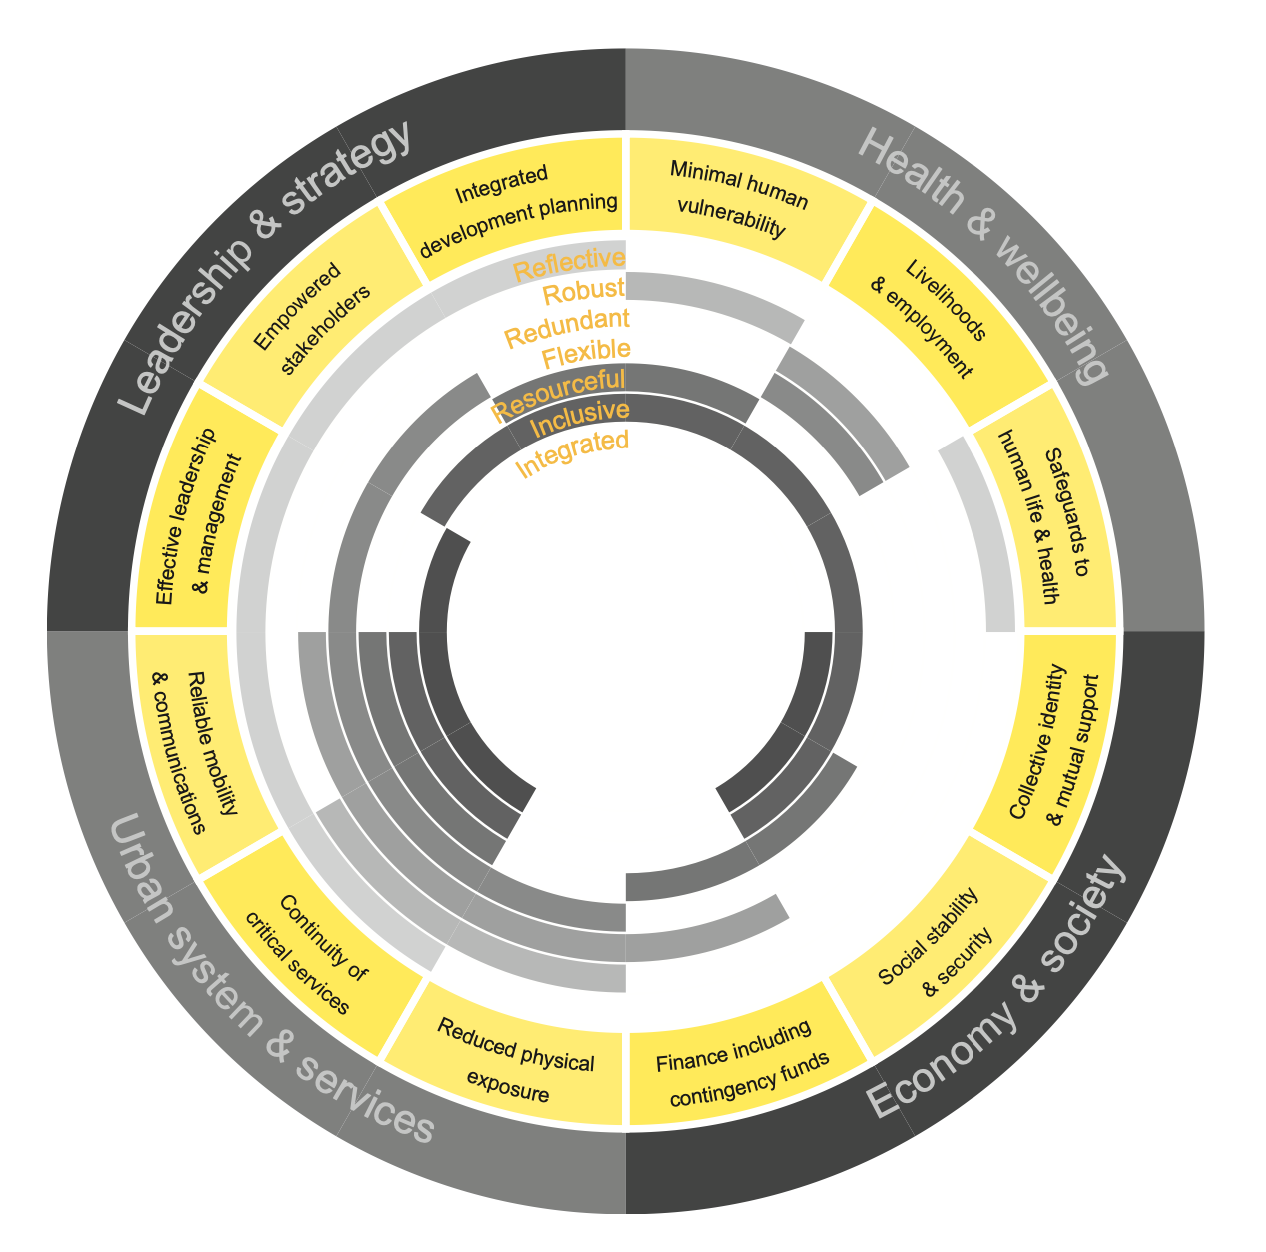
\includegraphics[width=4.16667in,height=4.16667in]{Imagen 1.png}
\caption{Resiliencia de una ciudad basada en sus características,
indicadores y categorías.}
\end{figure}

\begin{figure}
\centering
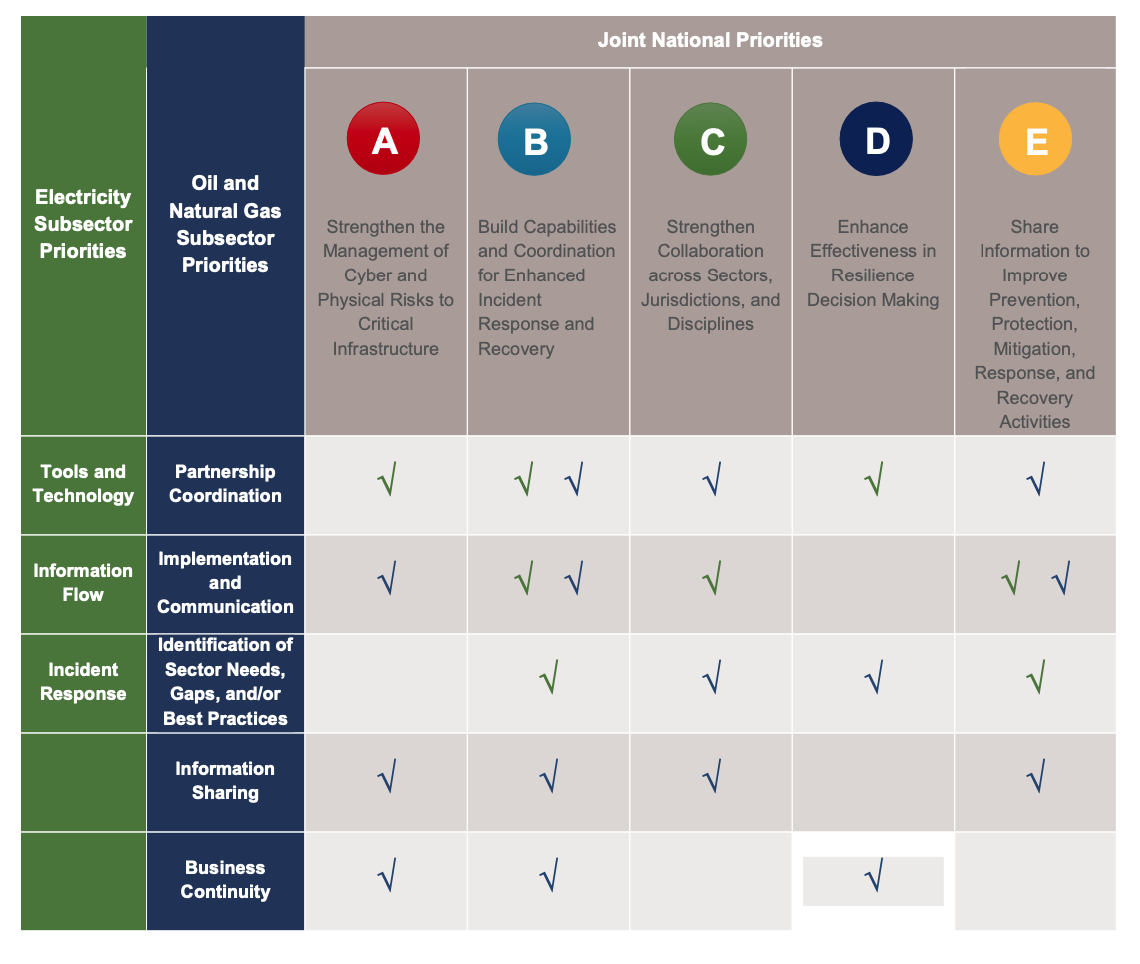
\includegraphics[width=5.20833in,height=5.20833in]{Imagen 2.png}
\caption{Prioridades del subsector eléctrico, subsector de petróleo y
gas, y el gobierno nacional.}
\end{figure}

\begin{figure}
\centering
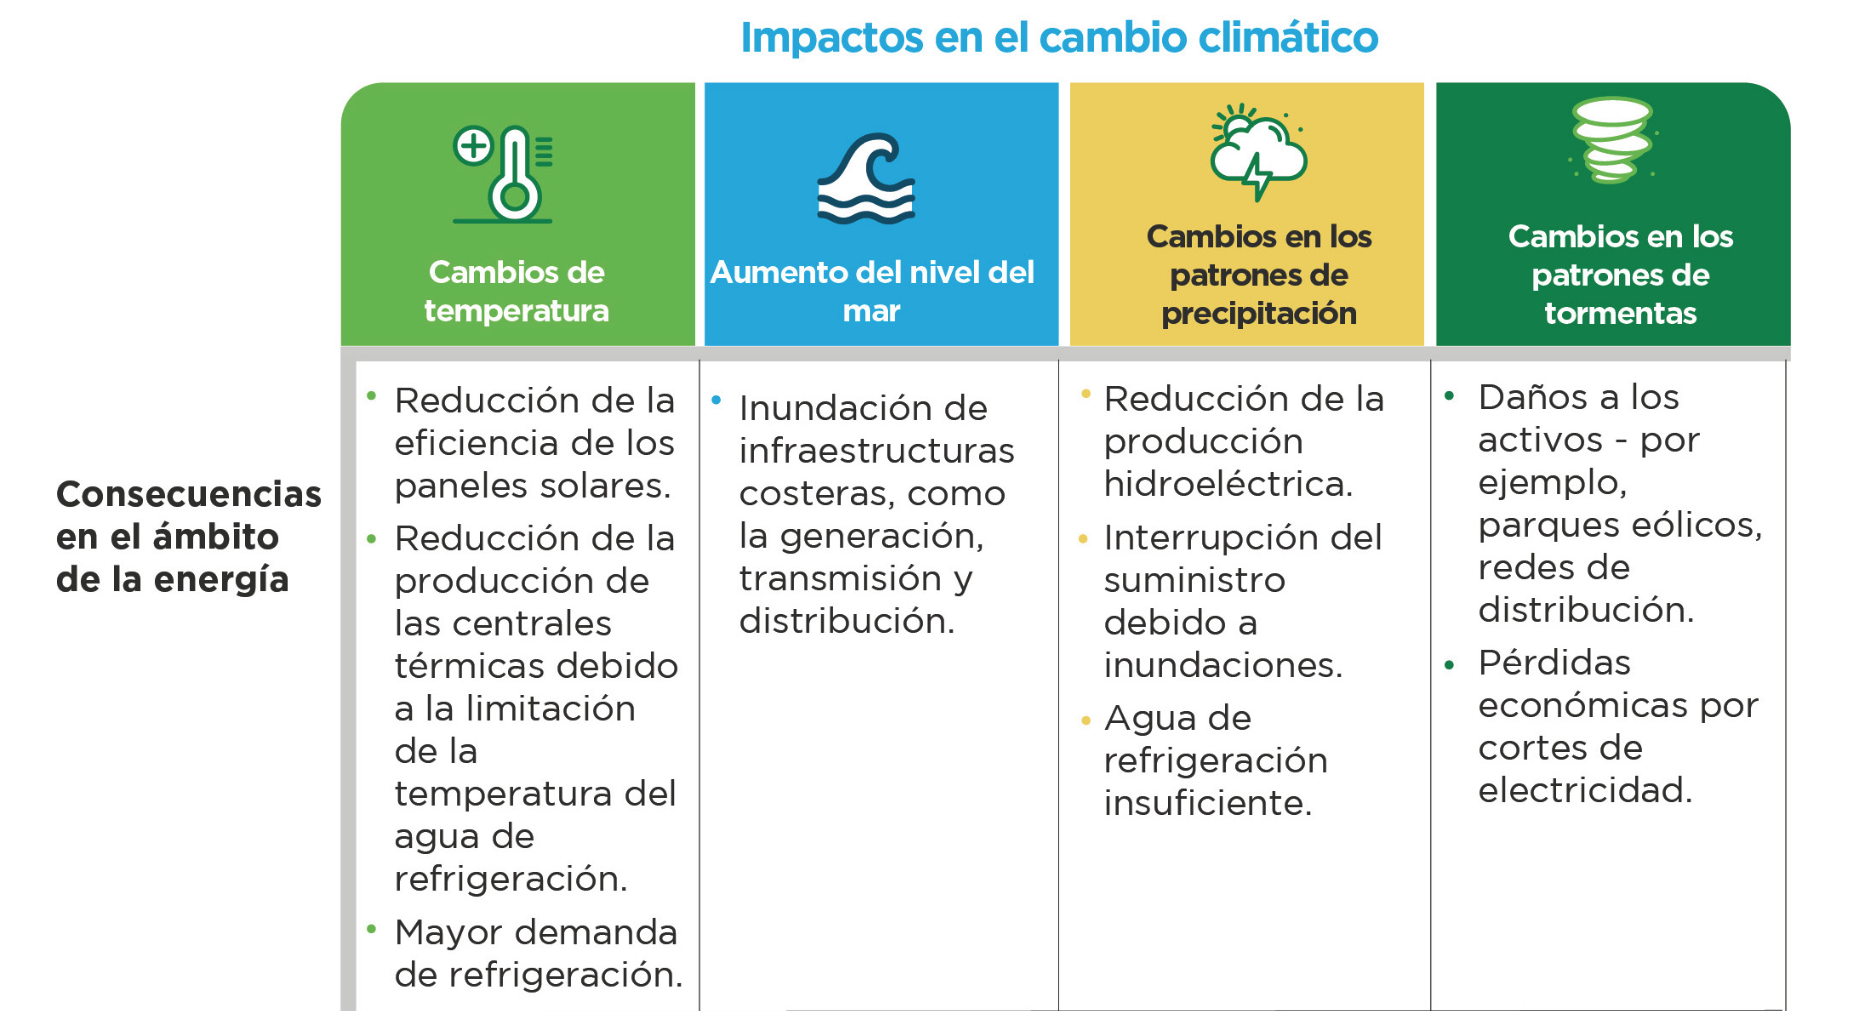
\includegraphics[width=7.29167in,height=4.16667in]{Imagen 3.png}
\caption{Consecuencias del cambio climático e impacto en el sector
energético.}
\end{figure}

\bibliographystyle{apa}
\bibliography{references.bib}


\end{document}
